\documentclass{article}
\usepackage[a4paper, left=3.5cm, right=3.5cm, top=4cm, bottom=4cm]{geometry}
\usepackage[T1]{fontenc}
\usepackage{minted}
\usepackage{mathabx}
\usepackage{graphicx}
\usepackage{float}
\usepackage{geometry}
\usepackage{longtable}
\usepackage{booktabs}
\usepackage{array}
\usepackage{rotating}

\begin{document}
\begin{center}
Planning Project - A Good Snowman is Hard to Plan\\
Matteo Paparo - Mat 264387
\end{center}
\clearpage
\section*{Introduction}
The 
following paper consists of a study regarding the use of \textit{PDDL Numeric}; specifically, the 
"A Good Snowman is Hard to Plan" problem was addressed.
The work is centered on the creation of snowmen, where several gradual conversions were made to the original domain. The choice was made to proceed by converting the most important components of the domain.
The objective of this analysis is to verify the impact of using PDDL Numeric on the proposed problem.
\section*{Domain}
The domain is represented on an \textit{n$\times$m} grid (not necessarily regular) where each 
cell can be covered in snow, and depending on the problem, there will be 3 to 6 snowballs for creating the snowmen.
With reference to the problem's objective, 3 different domains were identified, for creating 
1 and 2 snowmen, respectively.\\ 
The rules to be followed are:
\begin{itemize}
    \item If a snowball passes over a snowy cell, and the snowball is not at its maximum size, it will increase in size;
\item It is possible to create a stack of snowballs if the ball on top is smaller than the ball below it;
\item To move a snowball, the player must be in a cell adjacent to the snowball.
If the destination cell is free, 
    or contains a larger snowball, then the snowball can be moved, and the player will move to the cell previously 
    occupied by the ball.
\end{itemize}
\textbf{Types, objects and fluents}\\
The objects considered are the following: \textit{loc, dir}, and \textit{ball}.
The \textit{loc} type represents the position of a grid cell.
The \textit{dir} type enumerates the four directions in which the character and the balls can move (up, down, left, right), and the \textit{ball} type defines all the balls present in the scenario.
\\ \\
To model the current state, in the basic domain, the following predicates were defined:
\begin{itemize}
    \item (snow ?l - loc): location \underline{l} is covered in snow;
\vspace{-0.15cm}
    \item (next ?from ?to - loc ?d - dir): locations
    \underline{from} and \underline{to} are adjacent;
location \underline{to} is in
    direction \underline{d} relative to \underline{from};\vspace{-0.15cm}
    \item (occ ?l - loc): location \underline{l} contains at least one ball;\vspace{-0.15cm}
    \item (char at ?l - loc): character is at location \underline{l};\vspace{-0.15cm}
    \item (ball at ?b - ball ?l - loc): ball \underline{b} is at location \underline{l};\vspace{-0.15cm}
    \item (ball size s ?b - ball): ball \underline{b} has small size;\vspace{-0.15cm}
    \item (ball size m ?b - ball): ball \underline{b} has medium size;\vspace{-0.15cm}
    \item (ball size l ?b - ball): ball 
\underline{b} has large size;\vspace{-0.15cm}
    \item (goal): the goal is satisfied.
\end{itemize}
\vspace{0.5cm}
\noindent
\textbf{Actions}\\
The actions considered are the following: \textit{move\_character}, which, as the name suggests, allows the character to move to an adjacent cell,
\textit{move\_ball}, which allows a snowball to be moved to an adjacent cell, and \textit{goal}, which allows checking if the goal has been reached.\\ \\
With reference to the original version, the following results were obtained\footnote{For solving the problems, the \textit{enshp-20} solver was used, and they were solved on a device with an Apple Silicon M3 processor and 16Gb of RAM}:
\begin{table}[H]
    \centering
    \begin{tabular}{|c|c|c|}
        \hline
    
    \textbf{Domain} & \textbf{Problems} & \textbf{Solved} \\
        \hline
        1 & 33 & 25 \\
        \hline
        2 & 13 & 1 \\
        \hline
    \end{tabular}
\end{table}
\section*{Conversion to PDDL Numeric}
The adaptation of the domain to PDDL Numeric was carried out gradually. Starting from the base domain, the most functional conversion was implemented, which was the conversion 
of the predicates concerning ball\_size into 
a numeric function. Specifically, to identify the three sizes (small, medium, and large) of the snowballs, three different values were 
assigned: 1 for small, 2 for medium, and 3 for large.
Subsequently, an adaptation of the grid definition methodology was carried out,
converting the relative predicate into two numeric functions to identify the cell with coordinates.
To conclude, a conversion with a different verification methodology for the creation of snowmen.\\ \\
In summary, we identify 3 different versions:\vspace{-0.15cm}
\begin{itemize}
    \item[1] \textbf{Goal}: which includes the conversion of predicates regarding the size of the snowballs and the goal;\vspace{-0.15cm}
    \item[2] \textbf{Coord}: which, in addition to the previous conversion, identifies locations with numeric coordinates;\vspace{-0.15cm}
    \item[3] \textbf{Count\_ball}: which, in addition to the first version, keeps track of the number of snowballs in each location.\vspace{-0.15cm}
\end{itemize}
\phantom{a}\\
\phantom{a}
\section*{Goal - version}
In the original domain, to differentiate the size of a snowball, 
three different predicates were used. With the conversion to PDDL Numeric,
these were synthesized into a single numeric function called \textit{ball\_size}.
It can take three different values: 1 for small balls, 2 for medium balls, and 3 for large balls.
Finally, the predicate regarding the goal was also converted into a numeric function.
In the case of creating one snowman, it assumes 
the value 1 if the snowman has been created.
This conversion takes on a different meaning for domains designed for creating multiple snowmen, as it keeps track of the number of snowmen created; in fact, it was renamed to \textit{snowman\_built}.\\
In this regard, two significant predicates were added:\vspace{-0.15cm}
\begin{itemize}
    \item (snowman\_at ?l - loc): location \underline{l} contains a snowman;
\vspace{-0.15cm}
    \item (ball\_used\_in\_snowman ?b - ball): ball \underline{b} is used in a snowman.
\vspace{-0.15cm}
\end{itemize}
This choice was made to make the problem's objective clearer, because in the original domain, 
for the creation of multiple snowmen, it was checked whether all the snowballs were distinct from each other and
occupied different locations in groups of three.
As the domain has been implemented, it is extendable to problems
designed for creating multiple snowmen.\\ \\
This is the simplest conversion, which reported very satisfactory results.
Of the 46 proposed problems, 33 yielded a solution.
In detail, we have:\\
\begin{table}[H]
    \centering
    \begin{tabular}{|c|c|c|}
        \hline
        \textbf{Domain} & \textbf{Problems} & \textbf{Solved} \\
        \hline
        1 & 33 & 31 \\
        \hline
        2 & 13 & 2 \\
        \hline
    \end{tabular}
\end{table}
\noindent
Compared to the original version, there was a slight increase in grounding time, 
but a reduction in all other metrics.\\
On average, a \textbf{Grounding Time} was reported for the \textbf{Basic} version of \textbf{71.44 msec} and for the \textbf{Goal} version of \textbf{104.76 msec}, but with a reduction in \textbf{Plan-Length} of \textbf{11 steps}.
\begin{figure}[H]
    \centering
    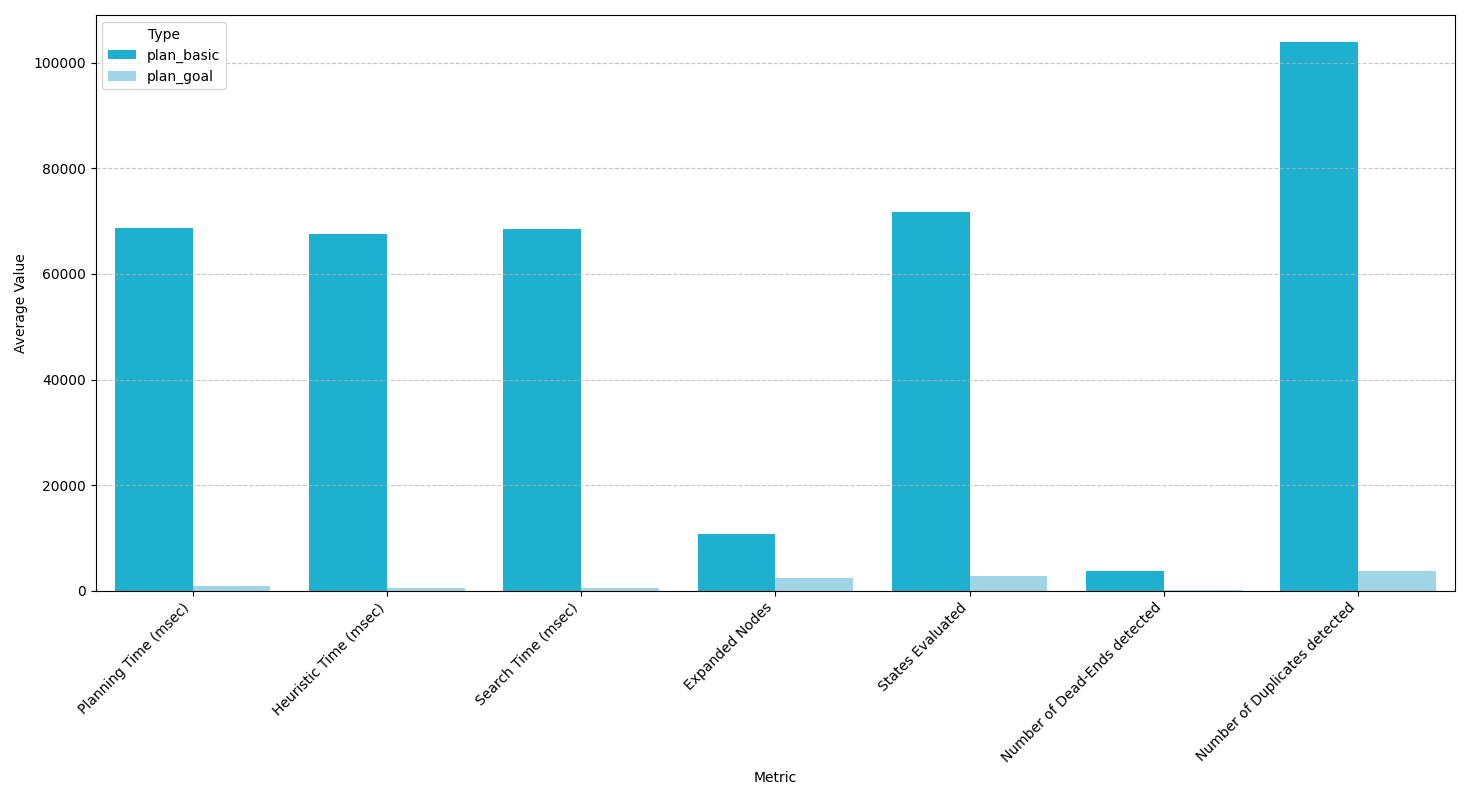
\includegraphics[width=1\textwidth]{/Users/matteo/Documents/Planning-Project/Report/images/basic_goal.png}
    \label{fig:goal}
\end{figure}
\noindent
From the graph, we can see a drastic reduction in the number of evaluated \textbf{States} and \textbf{Duplicates},
 which leads to a decrease in solving times, thus an optimization of the original domain.
\begin{figure}[H]
    \centering
    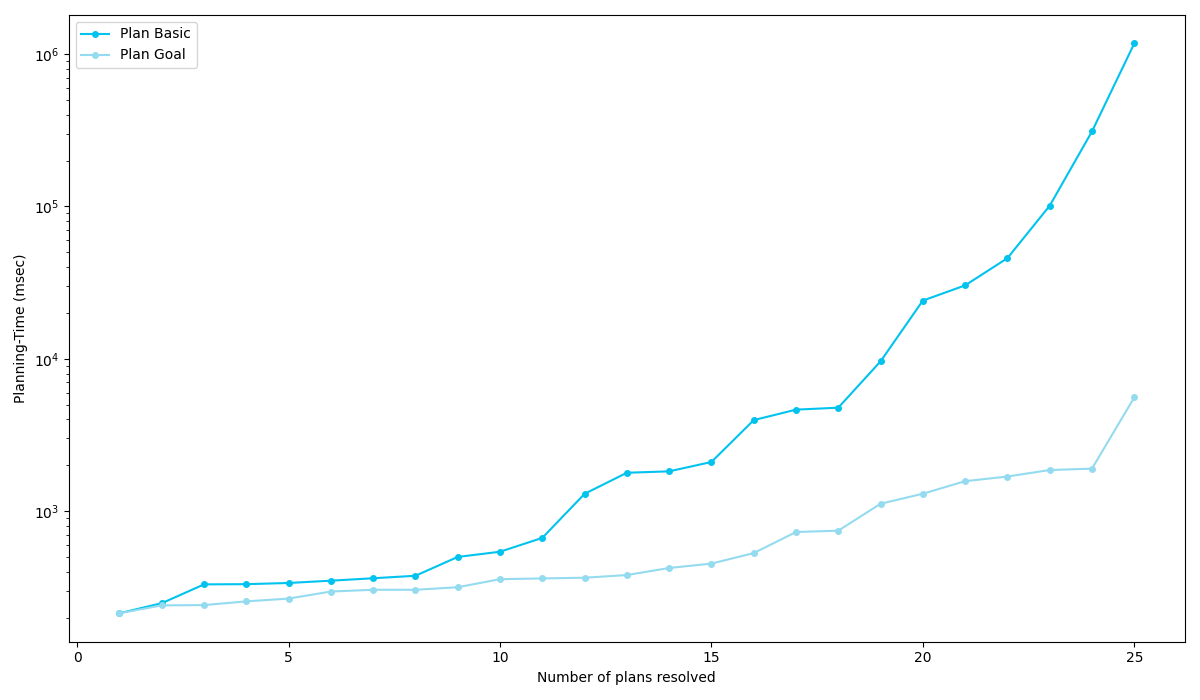
\includegraphics[width=1\textwidth]{/Users/matteo/Documents/Planning-Project/Report/images/time_basic_goal.png}
    \label{fig:goal_states}
\end{figure}
\noindent
From the following graph\footnote{This is not a comparison between the authors' plans}, it can be noted how the \textbf{Goal} version's \textbf{Planning Time}, as the number of solved plans increases, 
has a much more contained trend compared to the \textbf{Basic} version, which has an exponential trend.
This is because the \textbf{Goal} version has a much smaller number of states and duplicates.
\section*{Coordinate - version}
The \textbf{Coordinate} version was created with the goal of reducing the complexity of grid initialization.
In the \textbf{Basic} version, the connection between the various locations is made 
with the use of the predicate 
\begin{center}
    (next ?from ?to - loc ?d - dir)
\end{center}
thus requiring, for each cell in the grid, the definition of a predicate for each direction.
In this version, instead, the choice was made to identify each grid cell with numeric coordinates, in order to define the locations with a numeric function.
\begin{center}
    (x-coord ?l - location) \hspace{0.5cm} and \hspace{0.5cm} (y-coord ?l - location)
\end{center}
This modification is significant for reducing the number of predicates,
as for problems defined on large grids, the number of predicates grows exponentially.\\
This version is an extension of the \textbf{Goal} version, as it maintains the previous modifications.
With reference to this version, of the 46 proposed problems, 30 yielded a solution.
In detail, we have:
\begin{table}[H]
    \centering
    \begin{tabular}{|c|c|c|}
        \hline
        \textbf{Domain} & \textbf{Problems} & \textbf{Solved}\\
        \hline
        1 & 33 & 28 \\
        \hline
        2 & 13 & 2\\
        \hline
    \end{tabular}
\end{table}
\noindent
On average, a \textbf{Grounding Time} was reported for the \textbf{Goal} version of \textbf{113.93 msec} 
and for the \textbf{Coordinate} version of a significant \textbf{3170.13 msec}, a very important value to consider.
Meanwhile, the plan length did not undergo significant variations.
\begin{figure}[H]
    \centering
    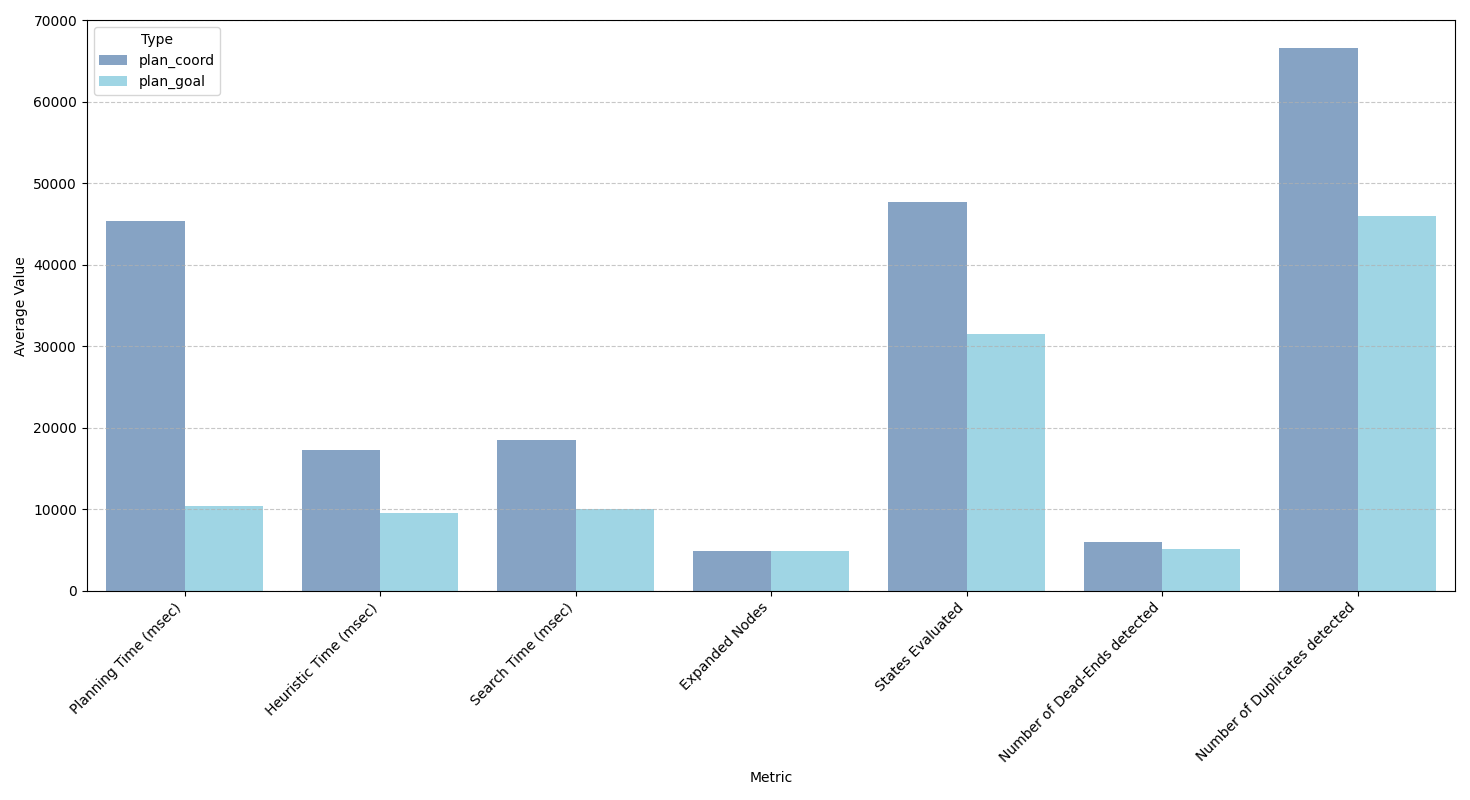
\includegraphics[width=1\textwidth]{/Users/matteo/Documents/Planning-Project/Report/images/goal_coord.png}
    \label{fig:coord}
\end{figure}
\noindent
From the graph, we can note a general increase in times.
The most significant data point is the disparity in the different \textbf{Planning Times}.
Specifically, on average, the \textbf{Goal} version has a better time of \textbf{4474.25 msec}, against the \textbf{46574.40 msec} of the \textbf{Coordinate} version, reporting values \textbf{10} times greater.
\begin{figure}[H]
    \centering
    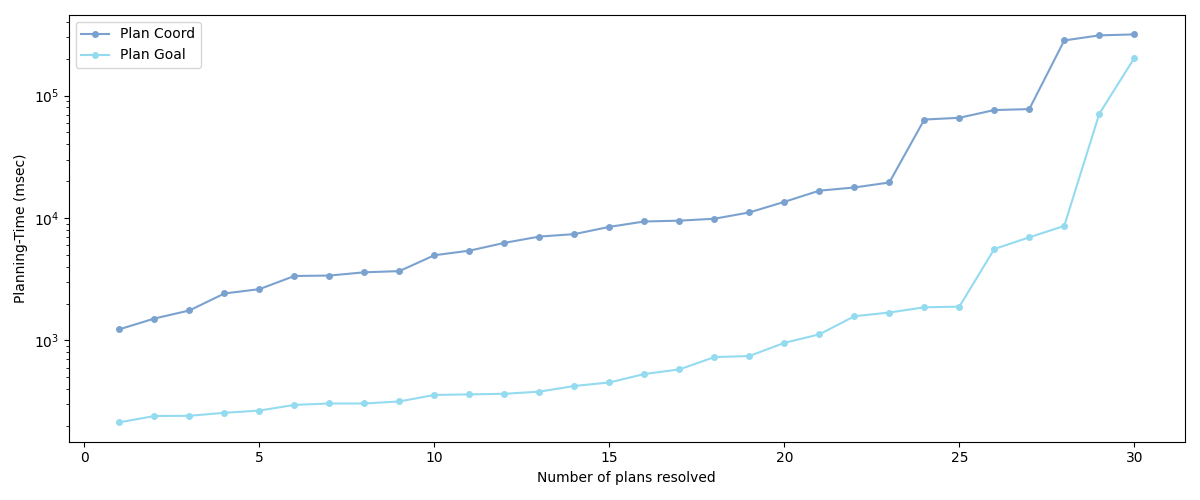
\includegraphics[width=1\textwidth]{/Users/matteo/Documents/Planning-Project/Report/images/time_goal_coord.png}
    \label{fig:coord_states}
\end{figure}
\noindent
The following graph highlights the difference between the \textbf{Planning Time} of the two versions, emphasizing the difference in times and their trend.
\section*{Count\_ball - version}
The \textbf{Count\_ball} version was created with the objective of tracking the number of snowballs in each location, with the secondary aim of avoiding the goal satisfiability check.
Due to the domain's structure, if three snowballs are in a single location, they will be ordered in descending size from bottom to top, ready for the creation of a snowman.
With the introduction of the function 
\begin{center}
    (ball\_count ?l - loc)
\end{center}
we avoid superfluous checks, reducing solving times.
This version is an extension of the \textbf{Goal} version, as it maintains the previous modifications.
With reference to this version, of the 46 proposed problems, 25 yielded a solution.
\begin{table}[H]
    \centering
    \begin{tabular}{|c|c|c|}
        \hline
        \textbf{Domain} & \textbf{Problems} & \textbf{Solved}\\
        \hline
        1 & 33 & 22 \\
        \hline
        2 & 13 & 3\\
        \hline
    \end{tabular}
\end{table}
\noindent
Compared to the \textbf{Goal} version, 
a reduction in \textbf{Grounding Time} was reported, respectively for the \textbf{Goal} version of \textbf{105.17 msec} and for the \textbf{Count\_ball} version of \textbf{79.25 msec}.
Furthermore, an increase in \textbf{Plan-Length} was reported; on average, the \textbf{Goal} version has a value of \textbf{52 steps} and the \textbf{Count\_ball} version has \textbf{66 steps}.
\begin{figure}[H]
    \centering
    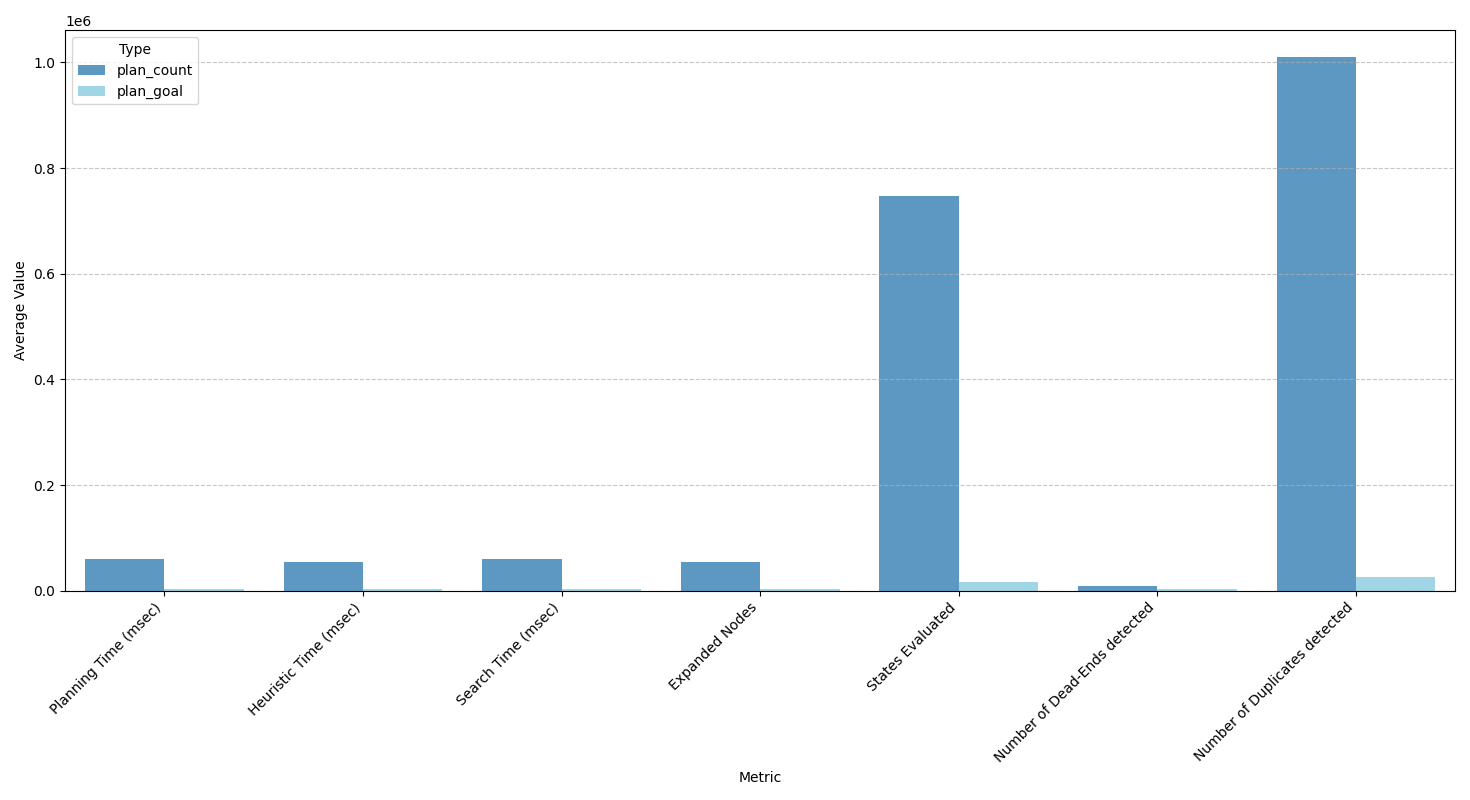
\includegraphics[width=1\textwidth]{/Users/matteo/Documents/Planning-Project/Report/images/goal_count.png}
    \label{fig:count_ball}
\end{figure}
\noindent
From the following graph, we can highlight the disparity in \textbf{States Evaluated} and \textbf{Duplicated States Evaluated} between the two versions.
In detail, we have that:
\begin{table}[H]
    \centering
    \begin{tabular}{|c|c|c|c|}
        \hline
        \textbf{Version} & \textbf{States Evaluated} & \textbf{Duplicated States Evaluated} \\
        \hline
        Goal & 16,561 & 748,227 \\
        \hline
        Count\_ball & 25,266 & 1,010,668 \\
        \hline
    \end{tabular}
\end{table}
\begin{figure}[H]
    \centering
    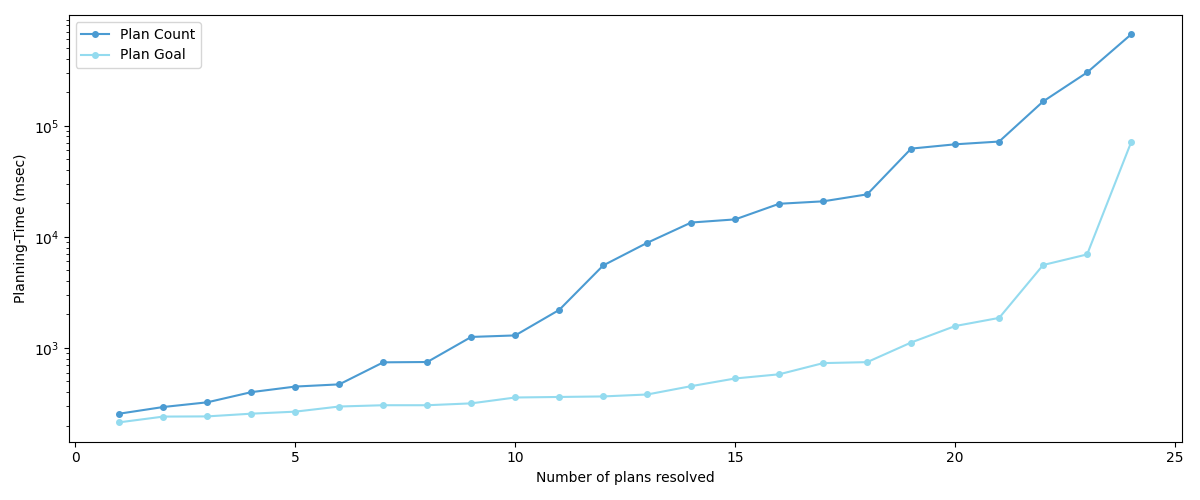
\includegraphics[width=1\textwidth]{/Users/matteo/Documents/Planning-Project/Report/images/time_goal_count.png}
   
 \label{fig:count_ball_states}
\end{figure}
\noindent
The following graph shows the trend of the \textbf{Planning Time} for the two versions, highlighting a more contained trend for the \textbf{Goal} version 
compared to the \textbf{Count\_ball} version, which, on the contrary, shows higher times even at a relatively low number of levels.
\section*{General Analysis}     
In general, the use of PDDL Numeric has led to very satisfactory results, as an increase in the number of solved problems and a reduction in solving times were achieved.
In particular, the Goal version showed an increase in the number of solved problems compared to the original version, while its extensions, namely the Coordinate and Count\_ball versions, reported 
negative aspects that unfortunately do not make them preferable to the Goal version.\\
From the Basic version to the Goal version, 9 more problems were solved, and the following graph highlights the reduced times compared to the other versions.
\begin{figure}[H]
    \centering
    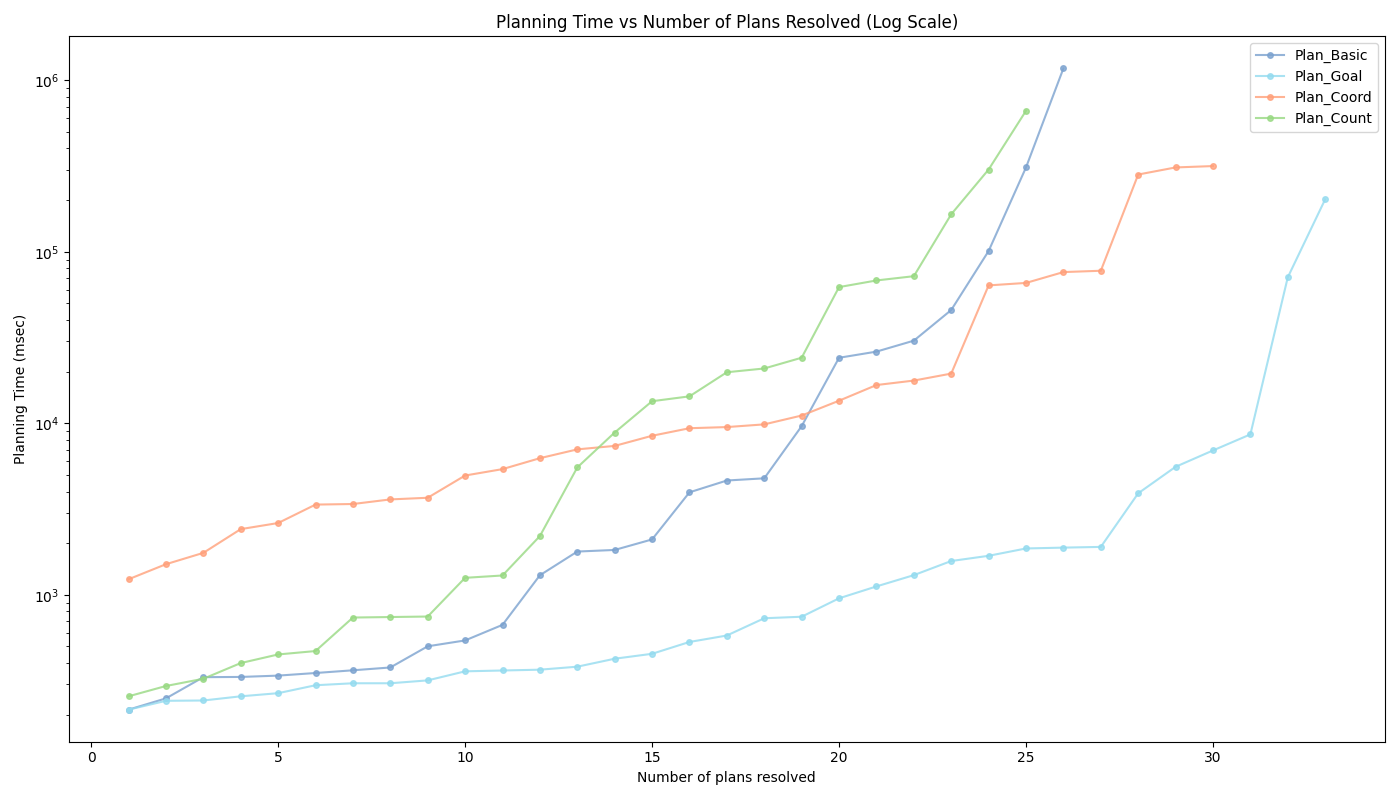
\includegraphics[width=1\textwidth]{/Users/matteo/Documents/Planning-Project/Report/images/all_time.png}
    \label{fig:all_versions}
\end{figure}
The following table summarizes the number of problems solved for each version:
\begin{table}[H]
    \centering
    \begin{tabular}{|c|c|c|c|}
        \hline
        \textbf{Version} & \textbf{Problem 1 and 2} & \textbf{Solved} \\
        \hline
        Basic & 33 - 13 & 25 - 1 \\
        \hline
        Goal & 33 - 
13& 31 - 2  \\
        \hline
        Coordinate & 33 - 13 & 28 - 2 \\
        \hline
        Count\_ball & 33 - 13 & 22 - 3 \\
        \hline
    \end{tabular}
\end{table}
\vspace{1cm}
In conclusion, each version highlights significant characteristics:
\begin{itemize}
    \item \textbf{Basic} with particularly long plans and a relatively high number of duplicates;
\item \textbf{Goal} has very fast planning with few expanded and duplicate nodes, but is not well-suited for complex scenarios;
\item \textbf{Coordinate} is balanced, has a medium-long plan while managing to keep duplicates under control, with moderate planning times;
\item \textbf{Count\_ball} is suitable for complex plans, but has a very high number of duplicates and long times; 
\end{itemize}


\end{document}